\documentclass{article}
\usepackage{tikz}
\usepackage{amsmath}
\usetikzlibrary{automata,positioning}

\begin{document}

\begin{figure}
\centering
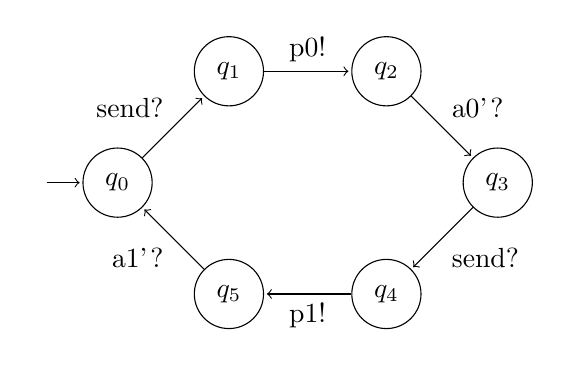
\begin{tikzpicture}[shorten >=1pt,node distance=2cm,on grid,auto]
  \path
  node[state,initial, initial text={}] (q_0)   {$q_0$}
  node[state] (q_1) [above right=of q_0] {$q_1$}
  node[state] (q_2) [right=of q_1] {$q_2$}
  node[state] (q_3) [below right=of q_2] {$q_3$}
  node[state] (q_4) [below left=of q_3] {$q_4$}
  node[state] (q_5) [left=of q_4] {$q_5$}
  ;
  \path[->]
  (q_0) edge  node {send?} (q_1)
  (q_1) edge  node {p0!} (q_2)
  (q_2) edge  node {a0'?} (q_3)
  (q_3) edge  node {send?} (q_4)
  (q_4) edge  node {p1!} (q_5)
  (q_5) edge  node {a1'?} (q_0)
  ;
\end{tikzpicture}
\caption{Input Sender}
\end{figure}


\begin{figure}
\centering
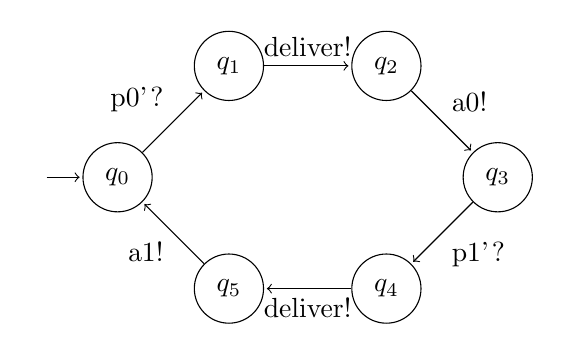
\begin{tikzpicture}[shorten >=1pt,node distance=2cm,on grid,auto]
  \path
  node[state,initial, initial text={}] (q_0)   {$q_0$}
  node[state] (q_1) [above right=of q_0] {$q_1$}
  node[state] (q_2) [right=of q_1] {$q_2$}
  node[state] (q_3) [below right=of q_2] {$q_3$}
  node[state] (q_4) [below left=of q_3] {$q_4$}
  node[state] (q_5) [left=of q_4] {$q_5$}
  ;
  \path[->]
  (q_0) edge  node {p0'?} (q_1)
  (q_1) edge  node {deliver!} (q_2)
  (q_2) edge  node {a0!} (q_3)
  (q_3) edge  node {p1'?} (q_4)
  (q_4) edge  node {deliver!} (q_5)
  (q_5) edge  node {a1!} (q_0)
  ;
\end{tikzpicture}
\caption{Input Receiver}
\end{figure}


\begin{figure}
\centering
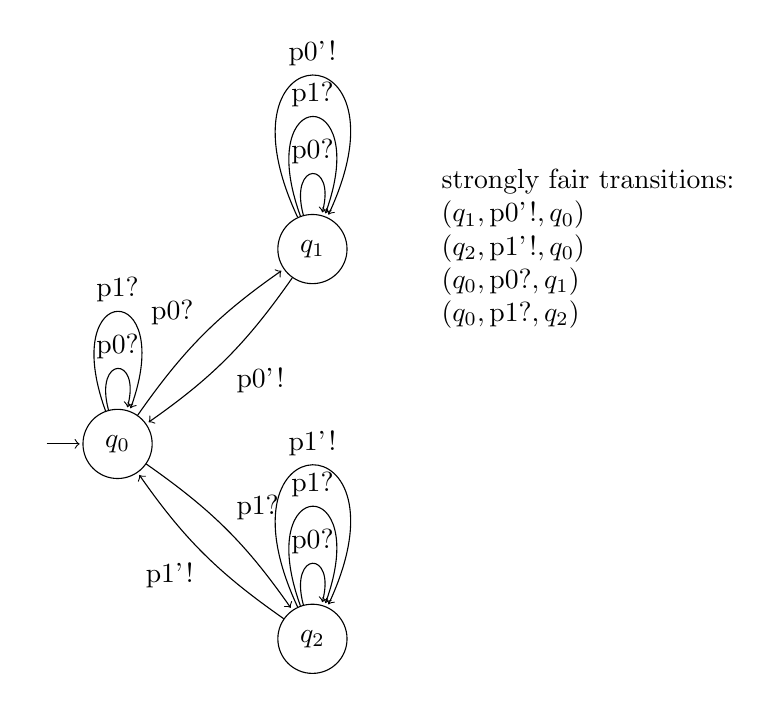
\begin{tikzpicture}[shorten >=1pt,node distance=3.5cm,on grid,auto]
  \path
  node[state,initial, initial text={}] (q_0)   {$q_0$}
  node[state,above right=of q_0] (q_1)  {$q_1$}
  node[state,below right=of q_0] (q_2)  {$q_2$}
  node[right=of q_1, align=left]
  {
    strongly fair transitions:\\
    $(q_1,\text{p0'!}, q_0)$\\
    $(q_2,\text{p1'!}, q_0)$\\
    $(q_0,\text{p0?}, q_1)$\\
    $(q_0,\text{p1?}, q_2)$
  }
  ;
  \path[->]
  (q_0) edge[out=55,in=215] node {p0?} (q_1)
  (q_1) edge[out=235,in=35] node {p0'!} (q_0)

  (q_0) edge[out=-35,in=125] node {p1?} (q_2)
  (q_2) edge[out=145,in=-55] node {p1'!} (q_0)

  (q_0) edge[loop above] node {p0?} (q_0)
  (q_0) edge[loop above, looseness=15, out=110, in=70] node {p1?} (q_0)

  (q_1) edge[loop above] node {p0?} (q_1)
  (q_1) edge[loop above, looseness=15, out=110, in=70] node {p1?} (q_1)
  (q_1) edge[loop above, looseness=18, out=115, in=65] node {p0'!} (q_1)

  (q_2) edge[loop above] node {p0?} (q_2)
  (q_2) edge[loop above, looseness=15, out=110, in=70] node {p1?} (q_2)
  (q_2) edge[loop above, looseness=18, out=115, in=65] node {p1'!} (q_2)
  ;
\end{tikzpicture}
\caption{Forward Channel}

\end{figure}


\begin{figure}
\centering
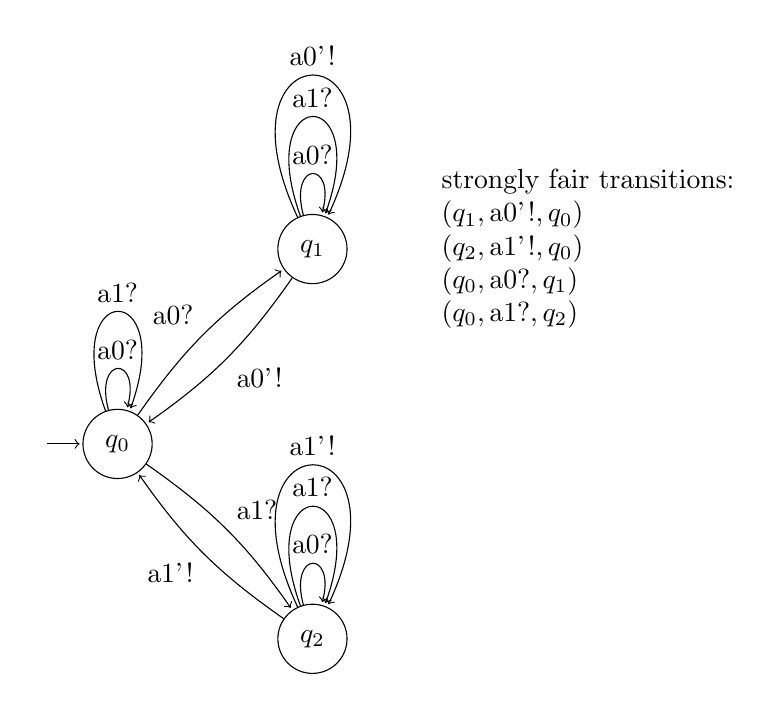
\begin{tikzpicture}[shorten >=1pt,node distance=3.5cm,on grid,auto]
  \path
  node[state,initial, initial text={}] (q_0)   {$q_0$}
  node[state,above right=of q_0] (q_1)  {$q_1$}
  node[state,below right=of q_0] (q_2)  {$q_2$}
  node[right=of q_1, align=left]
  {
    strongly fair transitions:\\
    $(q_1,\text{a0'!}, q_0)$\\
    $(q_2,\text{a1'!}, q_0)$\\
    $(q_0,\text{a0?}, q_1)$\\
    $(q_0,\text{a1?}, q_2)$
  }
  ;
  \path[->]
  (q_0) edge[out=55,in=215] node {a0?} (q_1)
  (q_1) edge[out=235,in=35] node {a0'!} (q_0)

  (q_0) edge[out=-35,in=125] node {a1?} (q_2)
  (q_2) edge[out=145,in=-55] node {a1'!} (q_0)

  (q_0) edge[loop above] node {a0?} (q_0)
  (q_0) edge[loop above, looseness=15, out=110, in=70] node {a1?} (q_0)

  (q_1) edge[loop above] node {a0?} (q_1)
  (q_1) edge[loop above, looseness=15, out=110, in=70] node {a1?} (q_1)
  (q_1) edge[loop above, looseness=18, out=115, in=65] node {a0'!} (q_1)

  (q_2) edge[loop above] node {a0?} (q_2)
  (q_2) edge[loop above, looseness=15, out=110, in=70] node {a1?} (q_2)
  (q_2) edge[loop above, looseness=18, out=115, in=65] node {a1'!} (q_2)
  ;
\end{tikzpicture}
\caption{Backward Channel}

\end{figure}

\begin{figure}
\centering
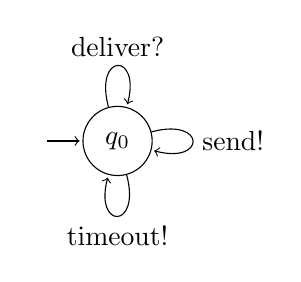
\begin{tikzpicture}[shorten >=1pt,node distance=3.5cm,on grid,auto]
  \path
  node[state,initial, initial text={}] (q_0)   {$q_0$}
  ;
  \path[->]
  (q_0) edge[loop above] node {deliver?} (q_0)
  (q_0) edge[loop right] node {send!} (q_0)
  (q_0) edge[loop below] node {timeout!} (q_0)
  ;
\end{tikzpicture}
\caption{Environment}
\end{figure}


\begin{figure}
\centering
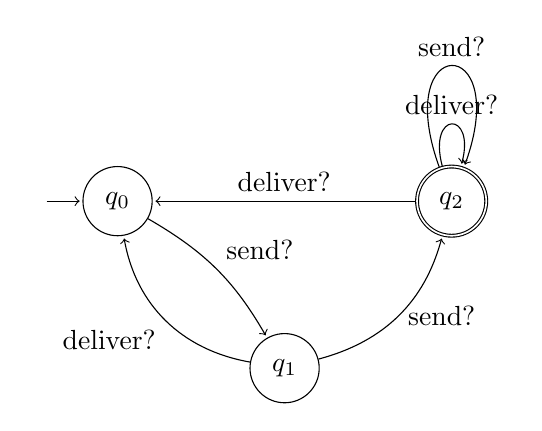
\begin{tikzpicture}[shorten >=1pt,node distance=3cm,on grid,auto]
  \path
  node[state,initial, initial text={}] (q_0)   {$q_0$}
  node[state] (q_1) [below right=of q_0] {$q_1$}
  node[state,accepting] (q_2) [above right=of q_1] {$q_2$}
  ;
  \path[->]
  (q_0) edge[out=-30,in=120] node {send?} (q_1)
  (q_1) edge[out=170,in=-80] node {deliver?} (q_0)

  (q_1) edge[bend right] node[right] {send?} (q_2)

  (q_2) edge[loop above] node {deliver?} (q_2)
  (q_2) edge[loop above, looseness=15, out=110, in=70] node {send?} (q_2)

  (q_2) edge node[above] {deliver?} (q_0)
  ;
\end{tikzpicture}
\caption{Safety Monitor}
\end{figure}


\begin{figure}
\centering
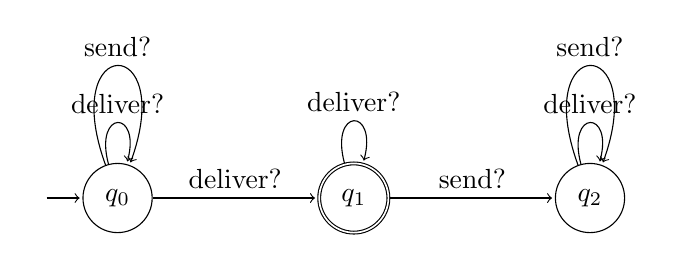
\begin{tikzpicture}[shorten >=1pt,node distance=3cm,on grid,auto]
  \path
  node[state,initial, initial text={}] (q_0)   {$q_0$}
  node[state,accepting] (q_1) [right=of q_0] {$q_1$}
  node[state] (q_2) [right=of q_1] {$q_2$}
  ;
  \path[->]
  (q_0) edge[loop above] node {deliver?} (q_0)
  (q_0) edge[loop above, looseness=15, out=110, in=70] node {send?} (q_0)

  (q_0) edge  node {deliver?} (q_1)

  (q_1) edge[loop above] node {deliver?} (q_1)

  (q_1) edge  node {send?} (q_2)

  (q_2) edge[loop above] node {deliver?} (q_2)
  (q_2) edge[loop above, looseness=15, out=110, in=70] node {send?} (q_2)
  ;
\end{tikzpicture}
\caption{Liveness Monitor send follows deliver}
\end{figure}

\begin{figure}
\centering
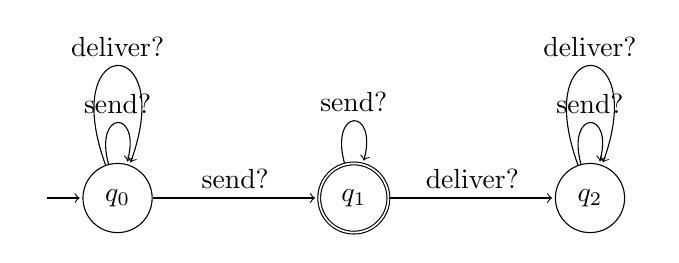
\begin{tikzpicture}[shorten >=1pt,node distance=3cm,on grid,auto]
  \path
  node[state,initial, initial text={}] (q_0)   {$q_0$}
  node[state,accepting] (q_1) [right=of q_0] {$q_1$}
  node[state] (q_2) [right=of q_1] {$q_2$}
  ;
  \path[->]
  (q_0) edge[loop above] node {send?} (q_0)
  (q_0) edge[loop above, looseness=15, out=110, in=70] node {deliver?} (q_0)

  (q_0) edge  node {send?} (q_1)

  (q_1) edge[loop above] node {send?} (q_1)

  (q_1) edge  node {deliver?} (q_2)

  (q_2) edge[loop above] node {send?} (q_2)
  (q_2) edge[loop above, looseness=15, out=110, in=70] node {deliver?} (q_2)
  ;
\end{tikzpicture}
\caption{Liveness Monitor deliver follows send}
\end{figure}


\begin{figure}
\centering
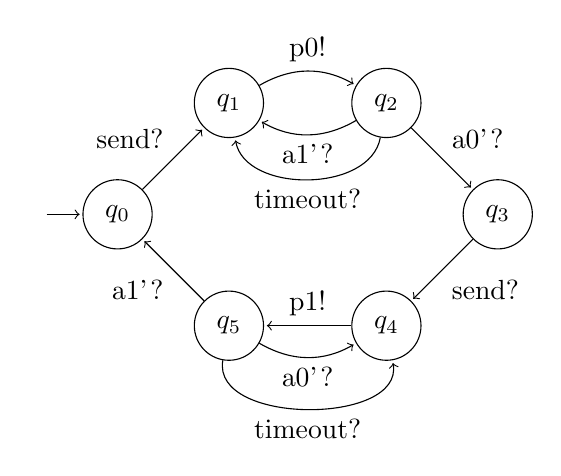
\begin{tikzpicture}[shorten >=1pt,node distance=2cm,on grid,auto]
  \path
  node[state,initial, initial text={}] (q_0)   {$q_0$}
  node[state] (q_1) [above right=of q_0] {$q_1$}
  node[state] (q_2) [right=of q_1] {$q_2$}
  node[state] (q_3) [below right=of q_2] {$q_3$}
  node[state] (q_4) [below left=of q_3] {$q_4$}
  node[state] (q_5) [left=of q_4] {$q_5$}
  ;
  \path[->]
  (q_0) edge  node {send?} (q_1)

  (q_1) edge[bend left]  node {p0!} (q_2)
  (q_2) edge[bend left]  node {a1'?} (q_1)
  (q_2) edge[out=260,in=280, looseness=1]  node {timeout?} (q_1)

  (q_2) edge  node {a0'?} (q_3)
  (q_3) edge  node {send?} (q_4)

  (q_4) edge  node[above] {p1!} (q_5)
  (q_5) edge[out=260,in=280, looseness=1]  node[below] {timeout?} (q_4)
  (q_5) edge[bend right]  node[below] {a0'?} (q_4)

  (q_5) edge  node {a1'?} (q_0)
  ;
\end{tikzpicture}
\caption{Solution Sender}
\end{figure}


\begin{figure}
\centering
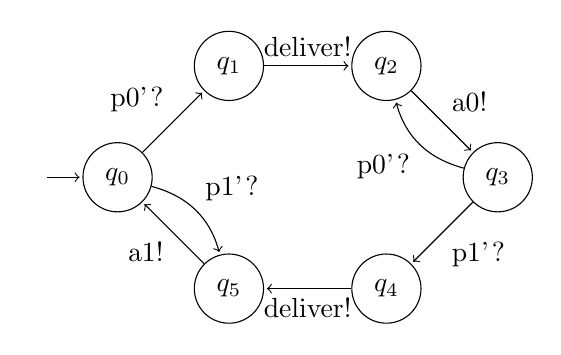
\begin{tikzpicture}[shorten >=1pt,node distance=2cm,on grid,auto]
  \path
  node[state,initial, initial text={}] (q_0)   {$q_0$}
  node[state] (q_1) [above right=of q_0] {$q_1$}
  node[state] (q_2) [right=of q_1] {$q_2$}
  node[state] (q_3) [below right=of q_2] {$q_3$}
  node[state] (q_4) [below left=of q_3] {$q_4$}
  node[state] (q_5) [left=of q_4] {$q_5$}
  ;
  \path[->]
  (q_0) edge  node {p0'?} (q_1)
  (q_1) edge  node {deliver!} (q_2)
  (q_2) edge  node {a0!} (q_3)
  (q_3) edge[bend left]  node {p0'?} (q_2)
  (q_3) edge  node {p1'?} (q_4)
  (q_4) edge  node {deliver!} (q_5)
  (q_5) edge  node {a1!} (q_0)
  (q_0) edge[bend left]  node {p1'?} (q_5)
  ;
\end{tikzpicture}
\caption{Solution Receiver}
\end{figure}


\end{document}